\chapter{Camera Model}
\label{chap:Camera Model}

The process of the camera mapping the coordinate points(the unit is meter) in the 3D world to the 2D image plane(the unit is pixel) can be described by a geometric model. There are many different models. The simplest of them is called the pinhole model. The pinhole model is a very common and effective model, it describes a beam of light after passing through the pinhole, its projection onto the image plane.

Now let's build a geometrically model for this simple pinhole model, which is shown in figure \ref{fig:pinhole_camera_model}. 

\begin{figure}[h!]
  \centering
  \begin{subfigure}[b]{0.6\linewidth}
    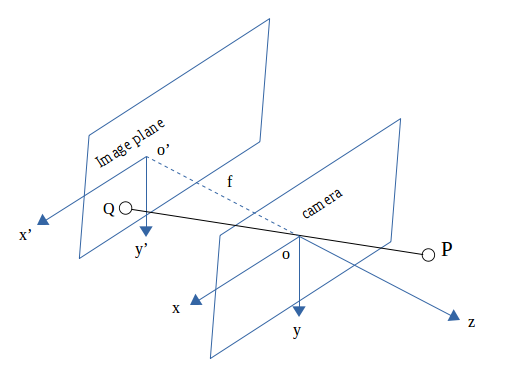
\includegraphics[width=\linewidth]{./fig/pinhole_camera.png}
    \caption{Camera coordinate system O-x-y-z}
  \end{subfigure}
  \begin{subfigure}[b]{0.3\linewidth}
    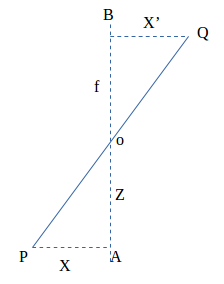
\includegraphics[width=\linewidth]{./fig/similar_triangles.png}
    \caption{Similar triangles}
  \end{subfigure}
  \caption{Pinhole camera model}
  \label{fig:pinhole_camera_model}
\end{figure}

\begin{figure}[h]
\centering
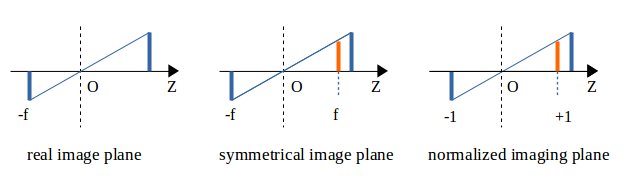
\includegraphics[scale=0.5]{./fig/3planes.png}
\caption{Real image plane, symmetrical image plane and normalized imaging plane}
\label{fig:3planes}
\end{figure}

We assume that o-x-y-z is camera coordinate system, z axis is pointing to the front of the camera, x axis is pointing to the right and y axis is pointing to down. The camera's optical center is \textit{o}, which is also the pinhole in the pinhole model. The real-world spatial point \textit{P} through the small pinhole is projected on physical image plane, the image point is \textit{Q}. We can assume that cartesian coordinate of \textit{P} is $\begin{bmatrix} X,Y,Z \end{bmatrix}^T$, \textit{Q} is $\begin{bmatrix} X',Y',Z' \end{bmatrix}^T$ and we assume that the distance from physical image plane to pinhole \textit{f}(camera focal length). Then, according to the triangle similarity theorems, we get equation \ref{eq:erla1}:

\begin{align}\label{eq:erla1}
&\frac{Z}{f} = -\frac{X}{X'} = -\frac{Y}{Y'}
\end{align}
The negative sign in equation \ref{eq:erla1} indicates that the image is inverted. In order to simplify this model, we can move the image plane to the front of the camera symmetrically, on the same side of the camera coordinate system together with the 3D spatial point. Now we can eliminate the negative sign as shown in figure \ref{fig:3planes}, make the equation more concise:
\begin{align}\label{eq:erla2}
&\frac{Z}{f} = \frac{X}{X'} = \frac{Y}{Y'}
\end{align}

After reforming equation \ref{eq:erla2}, we get the following equation which is equal to equation \ref{eq:erl5}(we will detailed explain the relationship between camera coordinate system and image plane coordinate system in section \ref{subsec:ccs_ics}):
\begin{equation}\label{eq:erla3}
 \left.\begin{aligned}
        X'=f\frac{X}{Z}\\
        Y'=f\frac{Y}{Z}
       \end{aligned}
 \right.
  \text{}
\end{equation}
Next the four plane coordinate systems in pinhole camera model and relationship between them would be introduced in the following sections:
\begin{enumerate}
\item Pixel plane coordinate system(u,v)
\item Image plane coordinate system(x,y)
\item Camera coordinate system($X_c,Y_c,Z_c$)
\item World coordinate system($X_w,Y_w,Z_w$)
\end{enumerate}

\section{The relationship between pixel plane coordinate system and image plane coordinate system}
Before determining their relationship, we can assume that the physical dimensions of each pixel in the u-axis and v-axis directions are dx and dy. Based on their model from figure \ref{fig:image_cs} we can derive the following formula:\\
\begin{align}\label{eq:erl1}
u & = \frac{x}{dx}+u_0
\end{align}
\begin{align}\label{eq:erl2}
v & = \frac{y}{dy}+v_0
\end{align}

\begin{figure}[h]
\centering
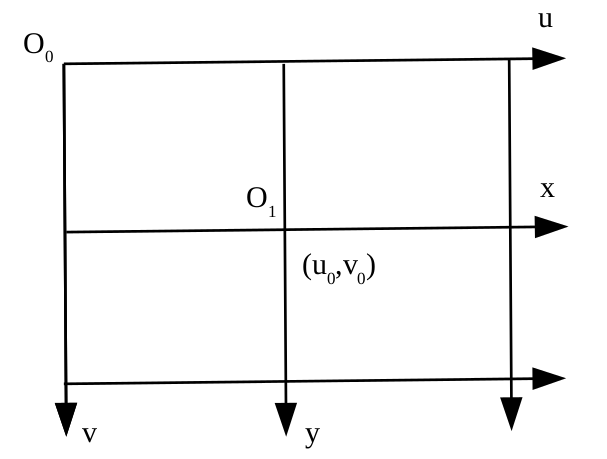
\includegraphics[scale=0.5]{./fig/image_cs.png}
\caption{Image plane coordinate system}
\label{fig:image_cs}
\end{figure}

dx, dy, u0, v0 are the parameters that we assume. dx, dy represent the actual size of the pixel on the light sensor chip. It is connected to the pixel coordinate system and the real size coordinate system. u0, v0 is the center of the image plane.

We can use the knowledge of linear algebra to represent equation \eqref{eq:erl1} and \eqref{eq:erl2} in matrix form:

\begin{equation}\label{eq:erl3}
\begin{bmatrix} u \\ v \\ 1 \end{bmatrix}
      = \begin{bmatrix} \frac{1}{dx} & 0 & u_0\\
                        0 & \frac{1}{dy} & v_0\\
                        0 & 0 & 1 \end{bmatrix}
        \begin{bmatrix} x \\ y \\1 \end{bmatrix}                 
\end{equation}

\section{The relationship between camera coordinate system and world coordinate system}

The relationship between these two coordinate systems we can rotate matrix \textit{R} and translation matrix \textit{t} to get the following relationship:
\begin{equation}\label{eq:erl4}
\begin{bmatrix} X_C \\ Y_C \\ Z_C \\ 1 \end{bmatrix}
      = \begin{bmatrix} R & t \\
                        0^T & 1 \end{bmatrix}
        \begin{bmatrix} X_W \\ Y_W \\ Z_W \\ 1 \end{bmatrix}                 
\end{equation}
In this equation, $R \in \mathbb{R}^{3\times3}$ rotates corresponding axes of each frame into each other and \textit{R} is orthogonal($R^TR = RR^T = I$), $t \in \mathbb{R}^{3\times1}$ defines relative positions of each frame.

\section{The Relationship between camera coordinate system and image plane coordinate system}
\label{subsec:ccs_ics}

In figure \ref{fig:ccs}, $O-X_CY_CZ_C$ is camera coordinate system and $o_1-xy$ is image plane coordinate system. According to the principle of triangle similarity theorems, we can derive following equations:

\begin{equation}\label{eq:erl5}
 \left.\begin{aligned}
        \frac{x}{f}=\frac{X_C}{Z_C}\\
        \frac{y}{f}=\frac{Y_C}{Z_C}
       \end{aligned}
 \right\} \Rightarrow
  \text{}
   \left\{\begin{aligned}
        Z_C \cdot x=f \cdot X_C\\
        Z_C \cdot y=f \cdot Y_C
       \end{aligned}
 \right.
  \text{}
\end{equation}

Also we can use the matrix form to represent this equations:
\begin{equation}\label{eq:erl6}
Z_C \begin{bmatrix} x \\ y \\ 1 \end{bmatrix}
      = \begin{bmatrix} f & 0 & 0 & 0 \\
                        0 & f & 0 & 0 \\
                        0 & 0 & 1 & 0 \\ \end{bmatrix}
        \begin{bmatrix} X_C \\ Y_C \\ Z_C \\ 1 \end{bmatrix}                 
\end{equation}

\begin{figure}[h]
\centering
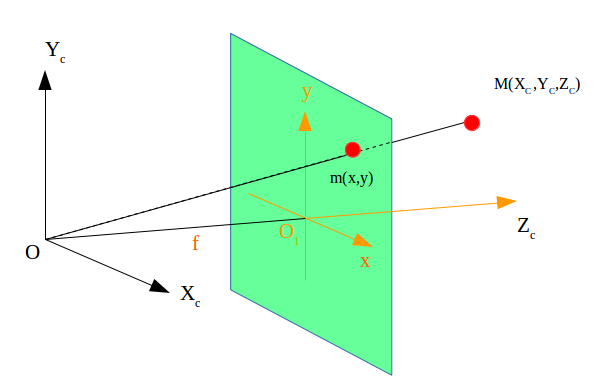
\includegraphics[scale=0.5]{./fig/ccs.png}
\caption{Image projection relationship}
\label{fig:ccs}
\end{figure}

And we can get the new formula from equations \ref{eq:erl3}, \ref{eq:erl4} and \ref{eq:erl6}:
\begin{equation}\label{eq:erl7}
Z_C \begin{bmatrix} u \\ v \\ 1 \end{bmatrix}
      = \underbrace{  
        \begin{bmatrix} \frac{1}{dx} & 0 & u_0\\
                        0 & \frac{1}{dy} & v_0\\
                        0 & 0 & 1 \end{bmatrix}
        \underbrace{                   
        \begin{bmatrix} f & 0 & 0 & 0 \\
                        0 & f & 0 & 0 \\
                        0 & 0 & 1 & 0 \\ \end{bmatrix}
        \underbrace{                 
        \begin{bmatrix} R & t \\
                        0^T & 1 \end{bmatrix}                                          
        \begin{bmatrix} X_W \\ Y_W \\ Z_W \\ 1 \end{bmatrix}
        }_\text{camera and world}    
        }_\text{projection relationship} 
        }_\text{pixel and image}                  
\end{equation}
So the camera intrinsic parameters can be described as a matrix \textit{K}:
\begin{equation}\label{eq:erl8}
K = \begin{bmatrix} f_x & 0 & u_0 & 0 \\
                    0 & f_y & v_0 & 0 \\
                    0 & 0 & 1 & 0 \\ \end{bmatrix}
  =
    \begin{bmatrix} \frac{1}{dx} & 0 & u_0\\
                     0 & \frac{1}{dy} & v_0\\
                     0 & 0 & 1 \end{bmatrix}                 
    \begin{bmatrix} f & 0 & 0 & 0 \\
                    0 & f & 0 & 0 \\
                    0 & 0 & 1 & 0 \\ \end{bmatrix}                  
\end{equation}
And \textit{R}, \textit{t} are the extrinsic parameters which denote the coordinate system transformations from 3D world coordinates to 3D camera coordinates. The extrinsic matrix can be described as:
$ \begin{bmatrix} R & t\\
                0^T & 1 \end{bmatrix}                  
$. Compared to the constant camera internal parameters, the extrinsic parameters will change with camera movement, \textit{R} and \textit{t} also denote the position of robot.

\begin{figure}[h]
\centering
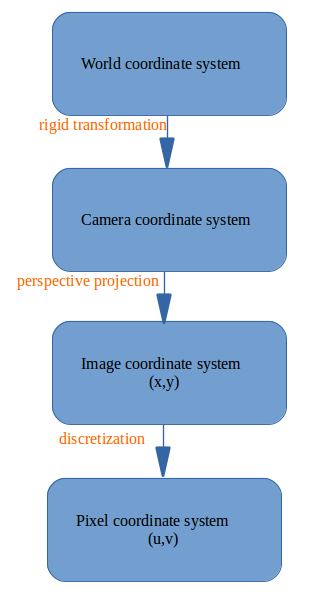
\includegraphics[scale=0.5]{./fig/4process.png}
\caption{Four coordinate systems and their relationships}
\label{fig:4process}
\end{figure}

\section{Camera distortion and image}
In geometric optics, distortion is a deviation from rectilinear projection; a projection in which straight lines in a scene remain straight in an image. It is a form of optical aberration\cite{wiki_do}.
% https://en.wikipedia.org/wiki/Distortion_(optics) 

We do not consider the camera distortion in this thesis.

In mathematics images can be described by a matrix. In the computer, they occupy a continuous disk or memory space and they can be represented by a two-dimensional array. Figure \ref{fig:image} shows a image, which height is 480 pixels and width is 640 pixels:
\begin{figure}[h]
\centering
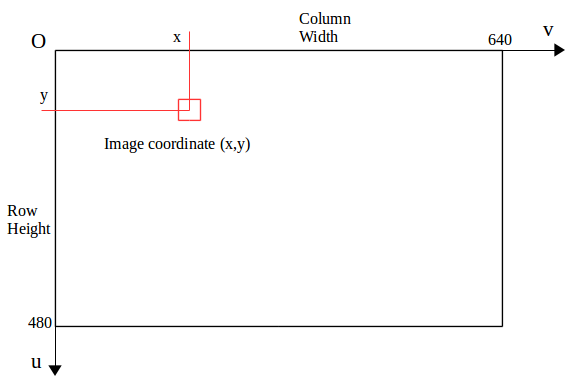
\includegraphics[scale=0.5]{./fig/image.png}
\caption{Image coordinate with 480 height and 640 width}
\label{fig:image}
\end{figure}

